% ---------------------------------------------------------------------------- %
% -------------------------- nevermind the preamble -------------------------- %
% ---------------------------------------------------------------------------- %
\documentclass[10pt,a4paper]{article}
\usepackage[a4paper, total={160mm, 240mm}]{geometry} % smaller margin %
\usepackage[utf8]{inputenc} % umlauts %
\usepackage[english]{babel} % validation %
\usepackage[autostyle]{csquotes}
\MakeOuterQuote{"}


\usepackage{hyperref}

\usepackage{enumitem}
\setlist[enumerate, 1]{label=(\alph*)}
\setlist[enumerate, 2]{label=\arabic*}

\usepackage{titlesec}
\titleformat{\section}[hang]{\small}{\textbf{Task \thesection:}}{.5em}{}

\usepackage{amsmath}
\usepackage{amssymb}

\usepackage{graphicx}
\usepackage[export]{adjustbox}
\usepackage[margin=4cm]{caption}

% ---------------------------------------------------------------------------- %
% -------------------------- nevermind the preamble -------------------------- %
% ---------------------------------------------------------------------------- %

\title{ \vspace{-3em}
        Assignment 01\\
		\small{\bf Digital Libraries and Foundations of Information Retrieval}\\
		\small{Winter semester 2022}}
\author{\small{\#\#\#\#\#\#\# Franka Brunen}, \small{1365848 Andreas Schneider}}
\date{}
\begin{document}
\setlength{\parskip}{6pt} % Remove paragraph first line h-indent and instead add v-margin %
\setlength{\parindent}{0pt}

\leftskip=1cm\rightskip=0.5cm % Indent paragraphs for readability %
\setlist[1]{leftmargin=2cm} % Indent first level of lists accordingly %

\maketitle

\section{\hfill Digital Preservation in Libraries\hfill 8+7 Points}
\begin{enumerate}
    \item \begin{itemize}
        \item The physical media will decay after some time\\
            $\rightarrow$ You can delay that to some extent with careful handling and proper storage measurements. For example paper is susceptible to high or low air humidity. UV radiation is another common factor that influences the lifetime of many physical media.
        \item Physically handling media results in physical stress\\
            $\rightarrow$ Covers of books could be protected by an additional wrapper. Optical media can be duplicated, so one could either only hand out copies or keep $>1$ lossless copy in storage. Access to important and vulnerable media could be restricted.
    \end{itemize}
    
    \item One compromise is to how lossless a copy will be.\\
    If the media is to be transformed to another data format, one can in most cases expect to lose information in the process. A digital recording of a vinyl will be contaminated with environmental conditions, like dust or air pressure and other influencing factors. In the best case, the resulting digital copy could be a perfect representation of the pickup during the time of recording, but can not be more than an approximation to the original piece of analog media.
    
    Duplicating digital media, on the other hand, is a completely lossless process.\\
    A concern one might still have is the possibility of all copies suffering from the same defect, like the corruption of a specific storage area, which would result in an unrecoverable loss of information. That can be solved by using multiple and different storage media, like a hard disk, flash memory, tape and optical discs.
    
    Optimally, there would be an infinitely scaling digital blueprint for every piece of media, like a scalable vector image or a \TeX\ typesetting definition, accompanied by an index of publication specifications which could include the printer, its firmware version, the used paper and other factors that had an influence on originally distributed copies.
\end{enumerate}



\section{\hfill Digitization of existing documents\hfill 5+5+5 Points}
\begin{enumerate}
    \item Video tape, like in the VHS cassette format, could be an interesting artifact to be digitized. I would not be surprised to find that some version of a movie or a recording might have exclusively been distributed via video tape.\\
    Another artifact of interest could be optical storage media, like the CD-DA or CD-ROM. Many pieces of music have their best or even only publicly available format in their distributed audio CDs. The same goes for software, foremost abandoned software products, that were distributed via CD-ROM.
    
    Other examples are floppy disks, BluRay Disks, LaserDisk, magnetic audio tape, photographic film, punched cards, or decommissioned proprietary formats like the NES cartridge.
    
    \item \begin{enumerate}
        \item Digitized media can be shared from and to anywhere at the speed of light.
        \item Digitized media can be losslessly duplicated without any cost to the original.
        \item Digitized media are machine-readable, meaning many media can be analyzed or augmented by the same algorithmic processes.
    \end{enumerate}
    
    \item You can analyze the color pigments and the structure of the paper of a document, or the details of a books binding to determine its place and time of origin. You lose that information at least to some degree when digitizing.
    
    Another analysis that is not possible with a digitized copy would be
    
    Not an analysis is the impression of a painting in a room, maybe even at a specific time with selected people. Or the shenanigans of some Audio CDs that would skip on older players, which can not really be replicated.
\end{enumerate}



\section{\hfill Analysis of publication titles\hfill 5+5+3+2 Points}
\begin{enumerate}
    \item Titles containing a colon appear more frequently now than in the past. But that is because documents in general appear more frequently now than in the past, as seen in figure \ref{fig:1}.
    \begin{figure}[h!!]
        \centering
        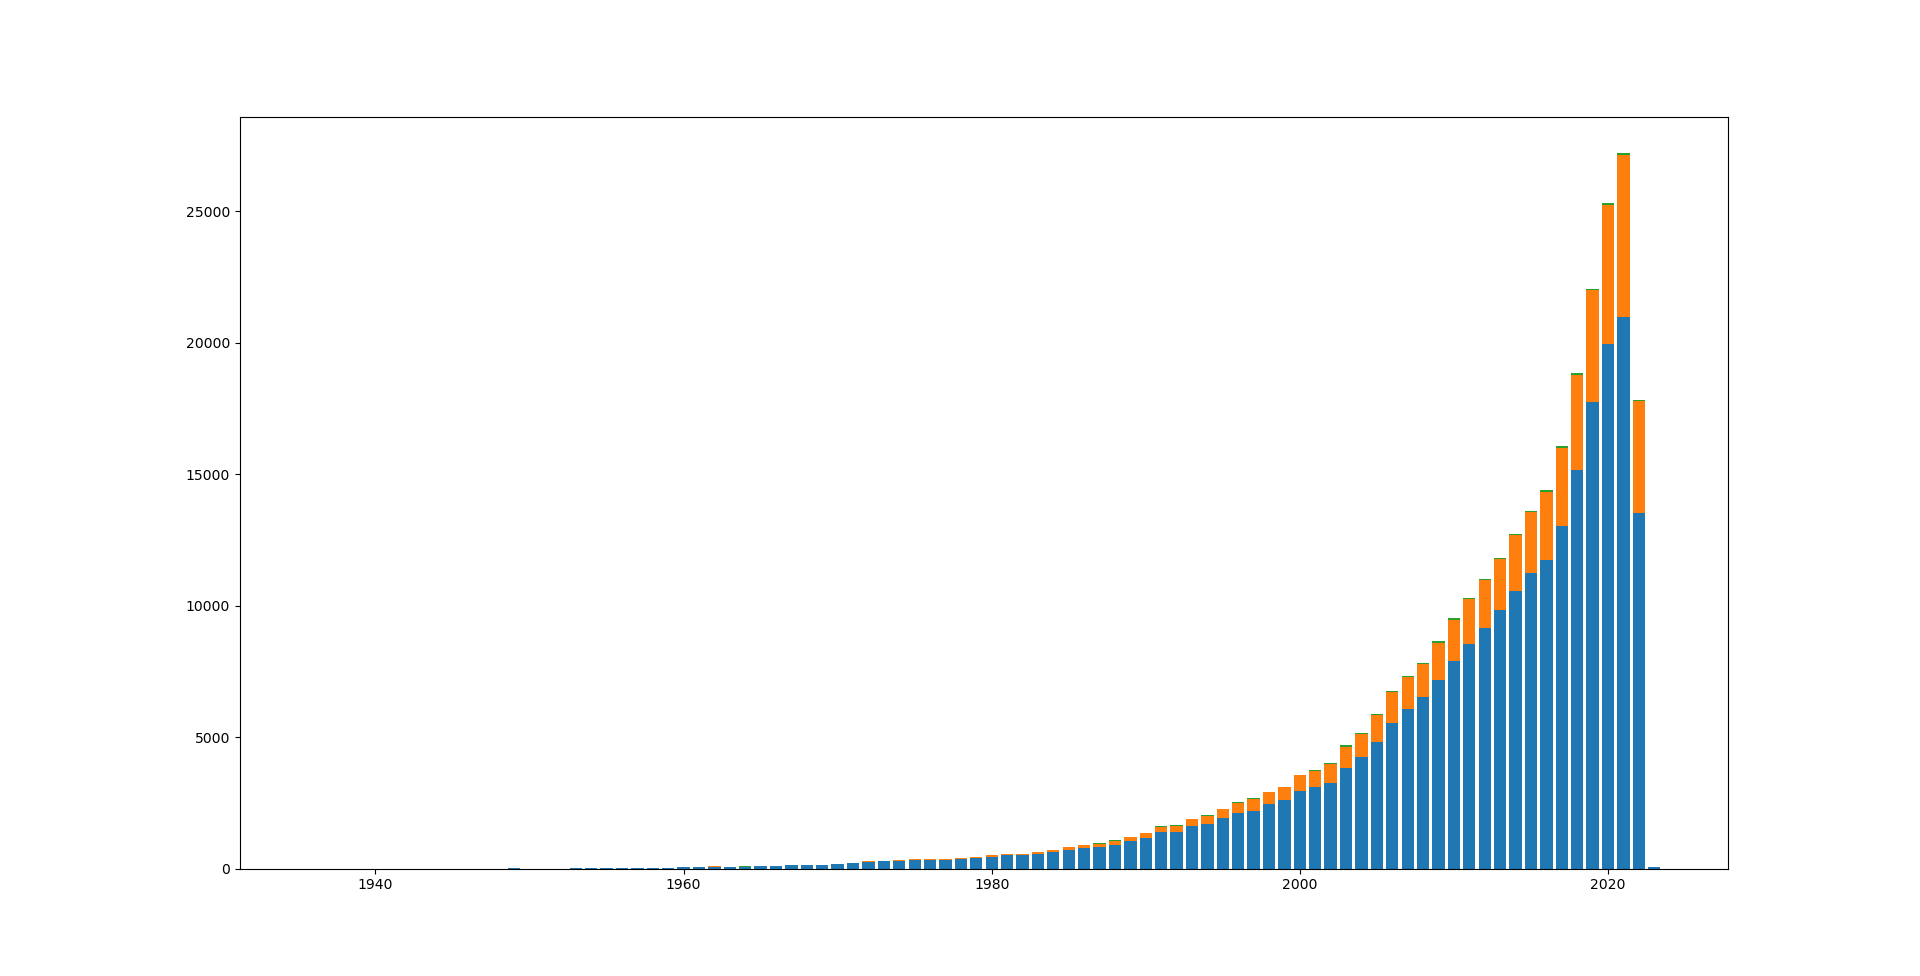
\includegraphics[width=0.8\textwidth]{Figure_1.png}
        \caption{Stacked bar graph of number of books titles with none, one and multiple colons per year}
        \label{fig:1}
    \end{figure}
    
    The relative bar plot makes for a more stable impression. Since the inception of this title style in the 1960s, it seems to have dropped not under 10\% representation, but also not gone way above 20\%, as seen in figure \ref{fig:2}.
    \begin{figure}[h]
        \centering
        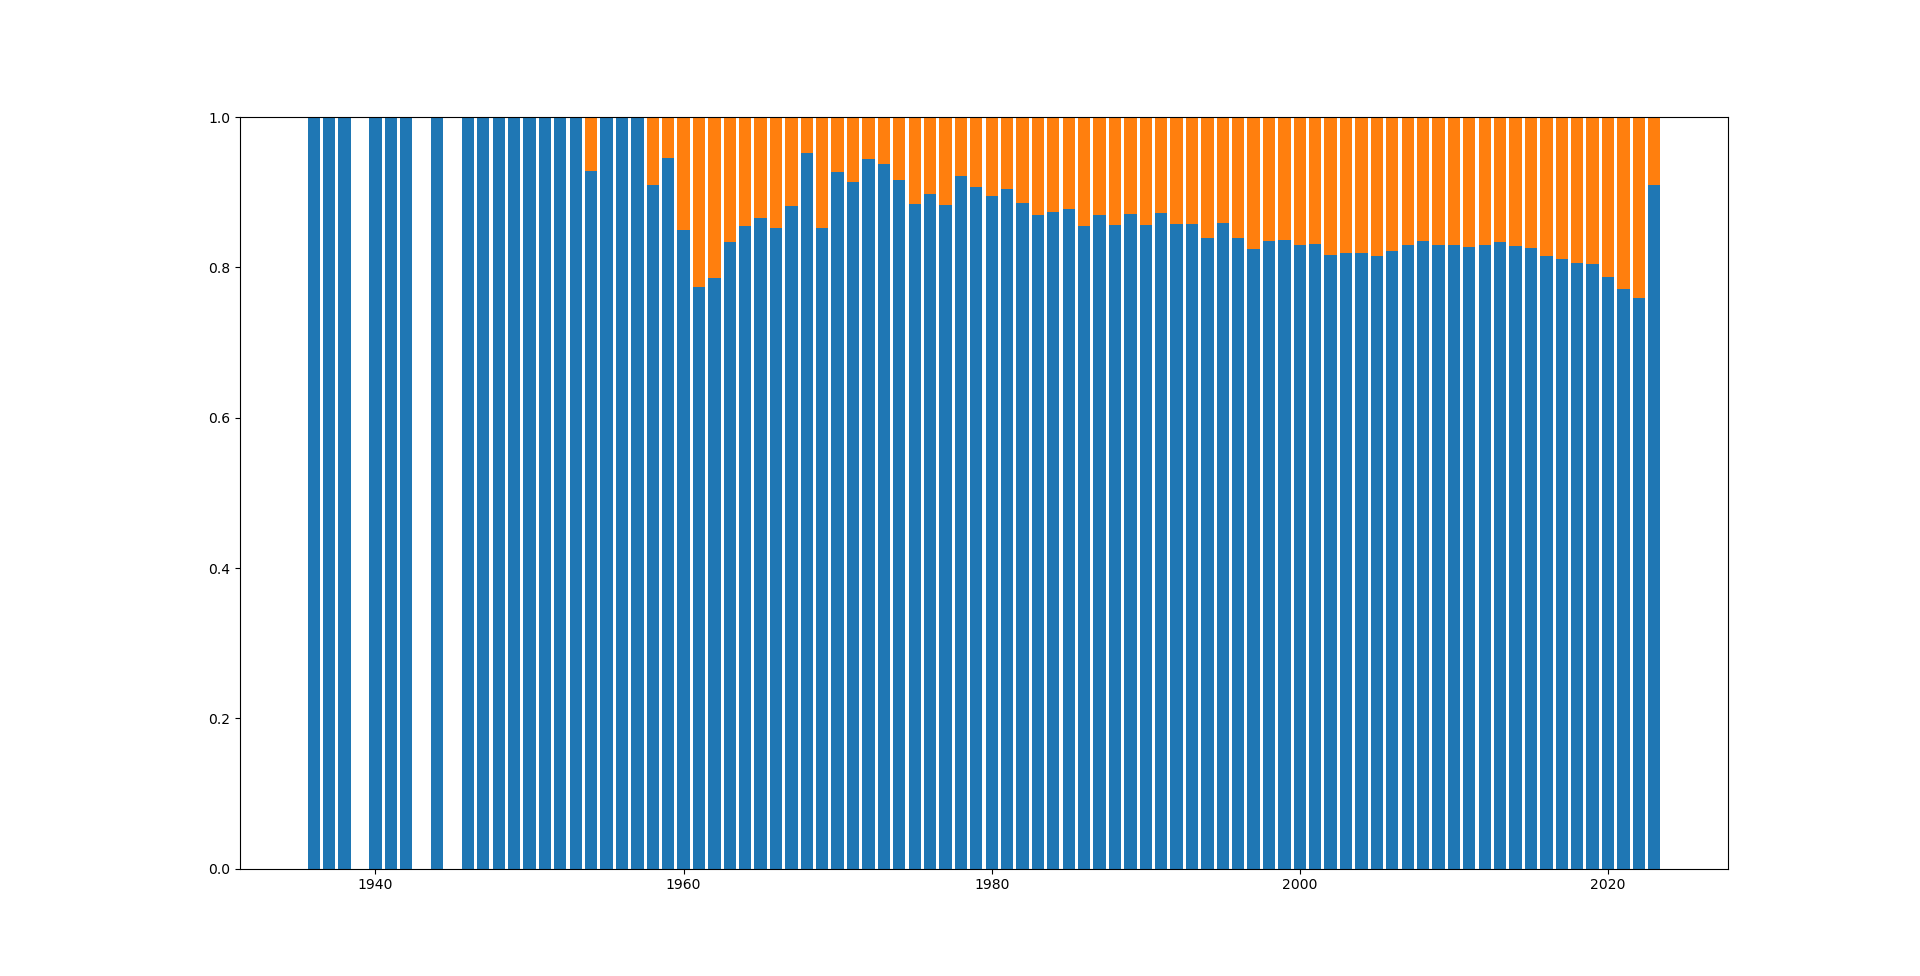
\includegraphics[width=0.8\textwidth]{Figure_2.png}
        \caption{Stacked bar graph of proportion of books titles with none and one or multiple colons per year}
        \label{fig:2}
    \end{figure}
    
    \item See figure \ref{fig:3}.
    \begin{figure}[h!]
        \centering
        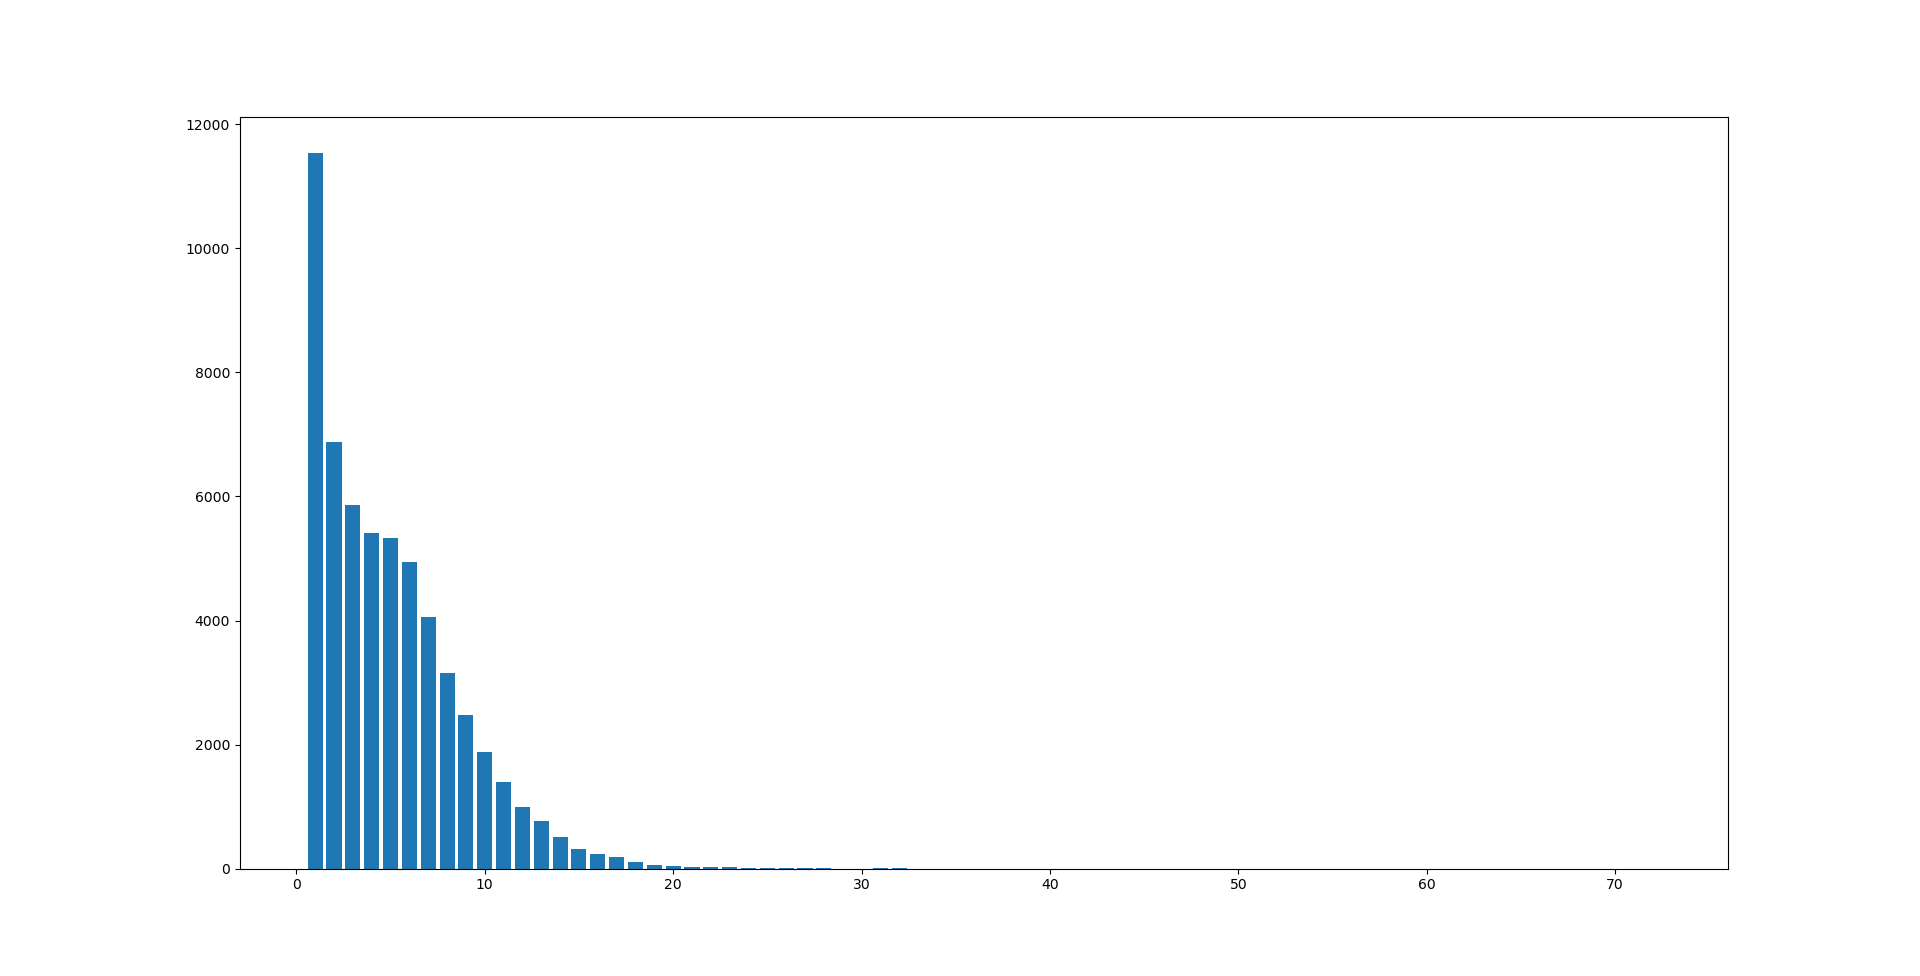
\includegraphics[width=0.8\textwidth]{Figure_3.png}
        \caption{Bar graph of frequency of word count before first colon}
        \label{fig:3}
    \end{figure}
    
    \item While looking at the rows by word count before the forst colon I noticed some odd data: One title had length 0 because it started with a colon. Another title had length 72 because the colon was only part of a URL at the end. I thought we were looking at titles here!
    
    Another interesting row was \#21654:
    \begin{verbatim}
['article',
 '2016',
 'R-Syst::diatom: an open-access and curated barcode database for diatoms
  and freshwater monitoring.']\end{verbatim}
    It was detected as 2-or-more-colons with two words before the first colon. I think detecting 'R-Syst::diatom' as one term would be preferable, but what other anomalies would that introduce, however one would achieve that detection? Is there a general agreement that 'Sainte-Mère-Église' is also one term?
    
    \item Some patterns in titles worth analyzing might me
    \begin{itemize}
        \item general word count,
        \item word length,
        \item use of quotes,
        \item use of abbreviations, or
        \item full sentences versus phrases.
    \end{itemize}
    
\end{enumerate}



\end{document}